\documentclass[]{spie}  %>>> use for US letter paper
%\documentclass[a4paper]{spie}  %>>> use this instead for A4 paper
%\documentclass[nocompress]{spie}  %>>> to avoid compression of citations

\renewcommand{\baselinestretch}{1.0} % Change to 1.65 for double spacing
 
\usepackage{amsmath,amsfonts,amssymb}
\usepackage{graphicx}
\usepackage[colorlinks=true, allcolors=blue]{hyperref}
\usepackage{float}

\title{Strategies for maximizing throughput in high-contrast ultraviolet apodized pupil lyot coronagraphs}


% Organizer
\author[a]{Jaren N. Ashcraft}

% Chefs Alphabetical by last name
\author[c]{Ramya Anche}
\author[e]{Jessica Gersh-Range}
\author[c]{Kyle van Gorkom}
\author[b]{Roser Juanola-Parramon}
\author[c]{Saraswathi Kalyani}
\author[a]{Maxwell A. Millar-Blanchaer}
\author[d]{A.J. Eldorado Riggs}

\affil[a]{Department of Physics, University of California, Santa Barbara, CA, 93106, USA}
\affil[b]{NASA Goddard Space Flight Center, Greenbelt, MD, 20771}
\affil[c]{Department of Astronomy and Steward Observatory, University of Arizona, 933 N. Cherry Ave., Tucson, AZ 85721, USA}
\affil[d]{NASA Jet Propulsion Laboratory, California Institute of Technology, 4800 Oak Grove Drive, Pasadena, CA 91109, USA}
\affil[e]{DM Telescopes LLC, Raleigh, NC 27615, USA}

\authorinfo{Further author information: (Send correspondence to J.N.A.)\\J.N.A.: E-mail: jarenashcraft@ucsb.edu}

% Option to view page numbers
\pagestyle{empty} % change to \pagestyle{plain} for page numbers   
\setcounter{page}{301} % Set start page numbering at e.g. 301
 
\begin{document} 
\maketitle

\begin{abstract}

\end{abstract}

% Include a list of keywords after the abstract 
\keywords{Manuscript format, template, SPIE Proceedings, LaTeX}

\section{Introduction}

NASA's Habitable Worlds Observatory aims to directly image and characterize $\approx 25$ habitable exoplanets to better constrain the occurence rate of worlds like our own. Among the characterization efforts includes an interest in the photometric characterization of exoplanets in the ultraviolet. The presence of ozone in a planet's atmosphere, leading to the very broad ozone absorption band, can help to determine at what stage in planetary evolution a planet is in. This scientific effort has ignited an interest in an unltraviolet coronagraph dedicated to exo-Earth characterization. The ultraviolet is a massive technical challenge, with particularly poor photon efficiency due to the high absorption of materials at shorter wavelengths. To solve this, many studies are investigating aluminum-based coatings with enhanced reflectivity in the ultraviolet. However, in this study we aim to leverage an additional degree of freedom to maximize throughput in the ultraviolet - the coronagraph masks themselves.

Because of the chromatic scaling of the point-spread function, we know that the diffraction-limited spot size of a distant point source is proportional to $\lambda/D$. This means that in the diffraction-limited regime, a coronagraph operating at $\lambda=250nm$ has twice the angular resolution as an equivalent coronagraph operating at $\lambda=500nm$. Equivalently, one could hold the angular resolution at a constant angle (say, 50mas), and derive that a 6m telescope's UV coronagraph has a $\approx5.8\lambda/D$ inner working angle (IWA), whereas the visible must operate with an IWA of $\approx2.9\lambda/D$ to observe targets at the same angular separation. In the world of pupil-plane coronagraphs, such as the Apodized Pupil Lyot Coronagraph (APLC) and Phase-apodized Pupil Lyot Coronagraph\cite{Por_2020} (PAPLC), the trade of throughput and IWA is well-known. By ``sacrificing" the uneccessary inner working angle in the UV, we can potentially gain a large degree of throughput that would ordinarily be lost to the coatings.

With respect to exoplanet detection and characterization, coronagraph core throughput is as important as mirror diameter. Increasing core throughput by a modest $10\%$ is almost as impactful to the coronagraph as increasing HWO's entrance pupil from $6.5$m to $7.1$m. In the UV, where a substantial amount of light is lost at every optic, maximizing core throughput is key to the success of an ultraviolet coronagraph. Herein we define throughput in accordance with Por 2020's definition\cite{Por_2020}, as the ratio of the encircled energies between the non-coronagraphic PSF ($\eta_0$) and the off-axis coronagraphic PSF ($\eta$), shown in Equation \ref{eq:throughput}, 

\begin{equation}
    T(\boldsymbol{k}, \lambda) = \frac{\eta(\boldsymbol{k}, \lambda)}{\eta_{0}(\boldsymbol{0}, \lambda)}.
    \label{eq:throughput}
\end{equation}

To be specific, $\eta_0$ does not include \emph{any} losses from the apodizer, focal plane mask, or Lyot stop.  

In this study, we report on an APLC design survey conducted to identify different degrees of freedom that can maximize throughput in the ultraviolet. In Section \ref{sec:design_methods} we illustrate the design methodologies used to optimize the coronagraph mask designs presented in this paper, which includes an open-source coronagraph design package called \texttt{dygdug} based on the \texttt{prysm} physical optics propagator. In Section \ref{sec:point_design} we build specifications to construct a ``point design" with which we will compare all other coronagraph masks to in order to quantitatively evaluate the gains in throughput that are possible. In Section \ref{sec:bandwidth_survey} we conduct our first design survey, where the \emph{bandwidth} of the APLC is surveyed to see how core throughput evolves with bandwidth in UV APLCs. In Section \ref{sec:ls_survey} we explore three different Lyot stop geometries to determine if one of these produces higher throughput solutions than the others. In Section \ref{sec:conclusions} we summarize the findings in this work and outline a plan for future design efforts in support of HWO.

\section{Design Methodology}
\label{sec:design_methods}
\textcolor{red}{Some blurb about AMPL / Gurobi, citation to prior work. AJ + Jessica please comment}
The first design methodology for the UV APLCs follows the same overall process that was used to design the shaped pupil coronagraph masks for the Nancy Grace Roman Space Telescope\cite{Gersh-Range_2022,Riggs_2017}.  This process consists of writing a linear program in AMPL\cite{AMPL} that maximizes a proxy for the coronagraph throughput (such as the clear area of the shaped pupil mask or the peak pixel value for an off-axis planet) subject to a set of constraints that includes the optical propagation equations and the contrast in the specified region of the image plane. This type of linear program is thoroughly described in Zimmerman et al. 2016\cite{Zimmerman_2016}, so the details are not reproduced here.

The design methodology that utilizes algorithmic differentiation is built in an entirely open-source environment based on the \texttt{prysm} numerical optics package. Written in Python, \emph{prysm} features hot-swappable GPU-accelerated optical propagation enabled by the \texttt{cupy} python package. \emph{prysm} is also natively differentiable, not relying on additional packages (e.g. \texttt{Jax}, \texttt{Pytorch}, \texttt{Tensorflow}) to compute the adjoint model of the objective function. The adjoints of the operations in a Lyot-type coronagraph are simple to implement, following the backpropagation logic in Jurling and Fienup\cite{Jurling:14}, so \texttt{prysm} has implemented these operations in its core propagation utilities. To extend \texttt{prysm}'s functionality to include coronagraph design, we introduce the free and open-source \texttt{dygdug} package. This package is an extension to \texttt{prysm} to include object-oriented optical systems, focal plane wavefront sensing, and critical to this work \emph{coronagraph design}. Building upon work presented in Ashcraft et al. 2025\cite{Ashcraft_2025}, we analytically derive the adjoint model for a Lyot-type coronagraph and extend the design problem to both amplitude- and phase- apodized Lyot coronagraphs (APLCs and PAPLCs, respectively). More detail about \texttt{dygdug} can be found in a forthcoming submission to the Journal of Open Source Software. For this study, preliminary optimizations are performed on a local workstation with an NVIDIA RTX 4090. Larger surveys were performed at the University of California, Santa Barbara Braid2 cluster on NVIDIA A100 GPU nodes, and NASA's Cabeus cluster on NVIDIA A100 GPU nodes. The ability to natively differentiate the coronagraph models is necessary for the high dimensionality of the problem ($\approx$262,000 variables), and running both the optimizer and the coronagraph models on GPUs using \texttt{cupy} makes for expeditious optimization. A typical coronagraph solution generated this way takes approximately 25 minutes to complete on the NVIDIA A100 GPU.

\subsection{On Throughput}
Given the purpose of this study, it is critical to be explicit about the definitions of ``throughput" used throughout. 

\begin{table}[H]
    \centering
    \begin{tabular}{c|c|c}
         Source & Definition & Notes  \\
         \hline
         Martinez 2010 \cite{martinez_2010} & N/A & \\
         N'Diyae et al. 2019\cite{Ndiaye_2019} & $\sum_{LS}^i I(x_i) / \sum_{EP}^i I(x_i)$ & Called ``transmitted energy" \\
         N'Diyae et al. 2019\cite{Ndiaye_2019} & $\eta(\mathbf{k}, \lambda) / \eta_0(0, \lambda) $ & Called ``encircled energy" \\
         Por 2020\cite{Por_2020} & $\eta(\mathbf{k}, \lambda) / \eta_0(0, \lambda) $ & Called ``core throughput" \\
         
         
    \end{tabular}
    \caption{A non-exhaustive review of the definitions of "throughput" used in prior coronagraph design studies.}
    \label{tab:placeholder}
\end{table}

\subsection{Building Specifications}

\subsubsection{Aperture}
For this study we baseline the LUVOIR-B Pupil. Since the aperture segmentation of HWO is not finalized, we choose an off-axis hexagonally segmented aperture (one geometry of interest for HWO) from a completed mission concept study. The methodology presented in this work is applicable to all aperture shapes, so the choice of the LUVOIR-B pupil is simply motivated by a precursor study to HWO. 

\subsubsection{Wavelength}
Strictly speaking, APLC optimization is wavelength-agnostic. The relative wavelengths included in the generally broadband optimization are what matter. However, the \texttt{prysm} optical propagator expresses propagation in units of physical distance (e.g. mm, $\mu$m), so an explicit wavelength is used in our propagation. We assume a center wavelength of $\lambda_c=350nm$, and utilize a $10\%$ bandwidth for our point design, with 5 wavelengths equally spaced across the band. In Section \ref{sec:bandwidth_survey} where we explore designs of progressively larger bandwidth, we hold a \emph{minimum} of 5 wavelengths across the band such that at minimum, two wavelengths are not spaced by more than $2\%$. Larger bandwidths include more wavelengths to accommodate for this.

\subsubsection{Dark Hole Extent and Focal Plane Mask}
Because the UV is restricted to a characterization mode, we assume some knowledge of the position of a theoretical exoplanet because it is detected in the visible. The trade-off between inner working angle and throughput is well-known\cite{Rouan2011}, but the relation between azimuthal extent and throughput is less-studied. Because the coronagraph presented here is a characterization-only coronagraph, we can theoretically gain some throughput by sacrificing the azimuthal extent of the dark hole. Following the Roman Coronagraph's characterization shaped-pupil coronagraph (SPC), we use a ``bowtie"-shaped dark zone. The APLC designs will have a symmetric dark hole (which naturally arises), and the PAPLC designs will only be required to have half the bowtie on one side of the focal plane. 

We first conduct a brief survey where the coronagraphs are optimized to maximize throughput and minimize contrast. The respective lagrange multipliers for throughput and contrast were not chosen judiciously. Rather, we simply aim to understand if there is a trend between different designs with the same cost function, where only the azimuthal extent of the dark hole and focal plane mask varies. Shown in Figure \ref{fig:azimuthal_study} are the results of a set of designs with discrete angular extents to sample between a small bowtie and a full $360^\circ$ dark hole.

\begin{figure}
    \centering
    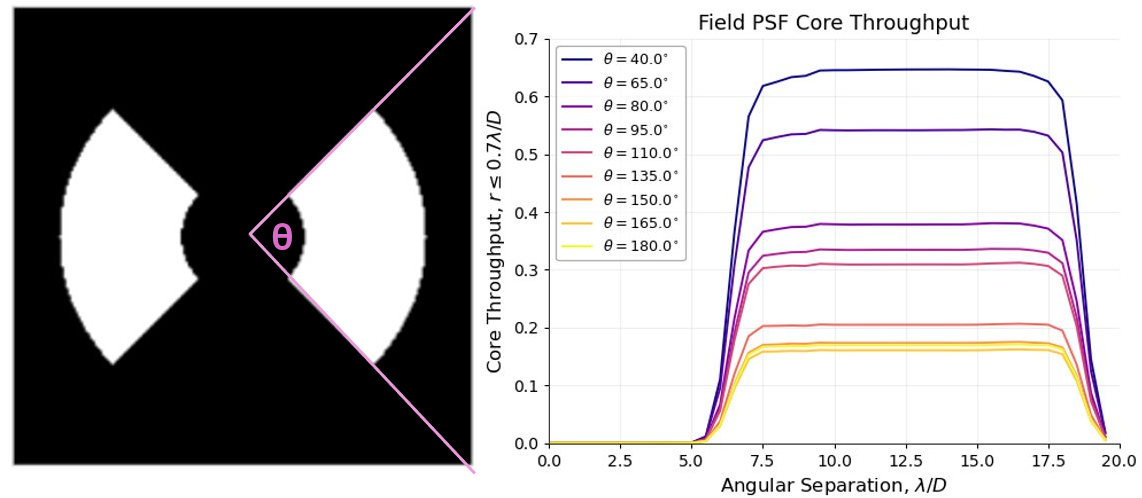
\includegraphics[width=0.9\linewidth]{azimuthal_throughput.png}
    \caption{Core throughput of APLCs subject to different azimuthal extents of the dark zone and focal plane mask for a fixed inner and outer working angle and bandwidth. We find generally that the azimuthal extent of the dark hole and focal plane mask are inversely proportional to the core throughput.}
    \label{fig:azimuthal_study}
\end{figure}

Figure \ref{fig:azimuthal_study} shows that there is a clear relation between core throughput and azimuthal extent. Intuitively, we understand that a smaller azimuthal extent means that there are fewer areas on the focal plane that are constrained to be high-contrast by the apodizer. In other words, less power from the apodization is required to destructively interfere light on the focal plane. For this characterization-only study, we choose a $65^\circ$ bowtie to leverage the relatively high core throughput achieveable, and be consistent with the Roman Coronagraph's bowtie SPC.

\subsubsection{Apodizer}
This study is concerned with the amplitude-apodizing APLCs, which operate by modifying the transmission at the entrance pupil of the coronagraph to create a region of high contrast on the focal plane. The broadband optimization of these APLC masks is conducted using the limited-memory and bounded version of the Broyden-Fletcher-Goldfarb-Shanno optimizer (L-BFGS-B), which supports exact box constraints on the optimization variables. Applying the box constraints allows us to force the APLC solution to be generally grayscale in the range of [0, 1]. There are no explicit constraints imposed to generate a binary APLC, but we find in the design surveys that binary APLCs have the highest throughput - and are therefore more ``optimal" than their grayscale counterparts.

\subsubsection{Lyot Stop}
For ease of alignment, we baseline a circular lyot stop at a radius of $0.95 \lambda_C / D_C$. This fractional radius was determined to have the highest core throughput over a grid-search of designs from a fractional radius of 0.8 to 0.99 in increments of 0.01. We will explore alternate Lyot stop geometries in a later section.

\subsubsection{Final Specifications}
Based on a mixture of specifications derived from the literature or empirical studies, we construct the following specifications in Table \ref{tab:specifications}.

\begin{table}[H]
    \centering
    \begin{tabular}{|l|c|c|c|}
    \hline
        \textbf{Specification} & \textbf{Value} & \textbf{Notes} & \textbf{Source} \\
    \hline
        Aperture & & LUVOIR-B Pupil &  \\
    \hline
        \phantom{ooo} Circumscribed diameter, $D_C$ [m] & 7.994 & & Juanola-Parramon et al\cite{Roser_2022} \\
        \phantom{ooo} Inscribed diameter [m] & 6.718 & & Juanola-Parramon et al\cite{Roser_2022} \\
        \phantom{ooo} Flat-to-flat distance [m] & 0.955 & & Juanola-Parramon et al\cite{Roser_2022} \\
        \phantom{ooo} Gap size [m] & 0.006 & & Juanola-Parramon et al\cite{Roser_2022} \\
    \hline
        Wavelength & & & \\
    \hline
        \phantom{ooo} Center Wavelength $\lambda_c$ [nm] & 350 & & Juanola-Parramon et al.\cite{roser_uv_2026} \\
        \phantom{ooo} Bandwidth $\frac{\Delta\lambda}{\lambda_c} \times 100$ [$\%$]& 10 & & Juanolla-Parramon et al. \cite{roser_uv_2026} \\
    \hline
        Dark Hole & &  & \\
    \hline
        \phantom{ooo} IWA [$\lambda_c / D_C$] & 6 & Based on HZ inner limits & Mamajek + Stapelfeldt\cite{mamajek_nasa_nodate}\\
        \phantom{ooo} OWA [$\lambda_c / D_C$] & 20 & Match visible OWA & \\
        \phantom{ooo} Angular Extent [$^\circ$] & $\pm$ 32.5 & & \\
    \hline
        Focal Plane Mask & & & \\
    \hline
        \phantom{ooo} Inner radius $r_{in}$ [$\lambda_c / D_C$] & 5.7 & & \\
        \phantom{ooo} Outer radius $r_{out}$ [$\lambda_c / D_C$] & 20 &  & \\
        \phantom{ooo} Angular Extent [$^\circ$] & $\pm$ 32.5 & & \\
    \hline
        Lyot Stop & & & \\
    \hline
        \phantom{ooo} Inner Diameter $D_{in}$ [$D_{in} / D_C$] & 0.0 & \textbf{Survey} & \\
        \phantom{ooo} Outer Diameter $D_{out}$ [$D_{out} / D_C$] & 0.95 & \textbf{Survey} & \\
    \hline
    Sampling & & & \\
    \hline
        \phantom{ooo} Pupil Plane Samples & 512 & & \\
        \phantom{ooo} Focal Plane Samples & 4px per $\lambda_c/D_C$ & & \\
    \hline
    \end{tabular}
    \caption{Specifications table for the ideal case, with no throughput maximization strategies employed other than an increased IWA}
    \label{tab:specifications}
\end{table}



\section{The Point Design}
\label{sec:point_design}

Based on the table defined in Section \ref{sec:design_methods} we conduct a joint minimization of a throughput ($T$) and contrast ($\mathcal{C}$) objective function given by Equation \ref{eq:objective},

\begin{equation}
    \mathcal{L}(\boldsymbol{\theta}) = \mathcal{C}_{DH}(\boldsymbol{\theta}) - \lambda \circ T(\boldsymbol{\theta}).
    \label{eq:objective}
\end{equation}

The objective function $\mathcal{L}$ is a function of the parameter vector $\boldsymbol{\theta}$, which correspond to the open area in the LUVOIR-B pupil. Using the box constraints avaialble via the L-BFGS-B optimizer we restrict $\boldsymbol{\theta} \in [0, 1]$. Because of the joint minimization, we need to search for the appropriate lagrange multiplier, $\lambda$, to produce a desireable design. The reader may think of the lagrange multiplier as the ``balance" between contrast and throughput that produces a desireable design. The APLC designs in this study took between 3-26 minutes to design on an NVIDIA A100 GPU. The ability to leverage high-performance computing systems allowed us to parallelize a grid search over the optimal lagrange multipliers and lyot stop radii at high resolution. When the lagrange multiplier was too high, the optimization exited quickly ($\lteq 1$ min), because the open aperture starting point is the maximal throughput solution. The more substantial optimizations that took between 3-26 minutes gradually dropped the contrast while maintaining throughput, with deeper contrasts tending to take more time to optimize. From this grid search, we are able to select the optimal combination of lagrange multiplier and lyot stop radii to produce a design that achieve $10^{-10}$ contrast at the inner working angle, and has the highest throughput.
The resulting APLC is the nominal design we use to compare across the different throughput maximization strategies, which we call the \emph{point design}%. The nominal contrast and core throughput, as well as a diagram of the coronagraph masks, are given in Figure \ref{fig:point_design}.

\begin{figure}
    \centering
    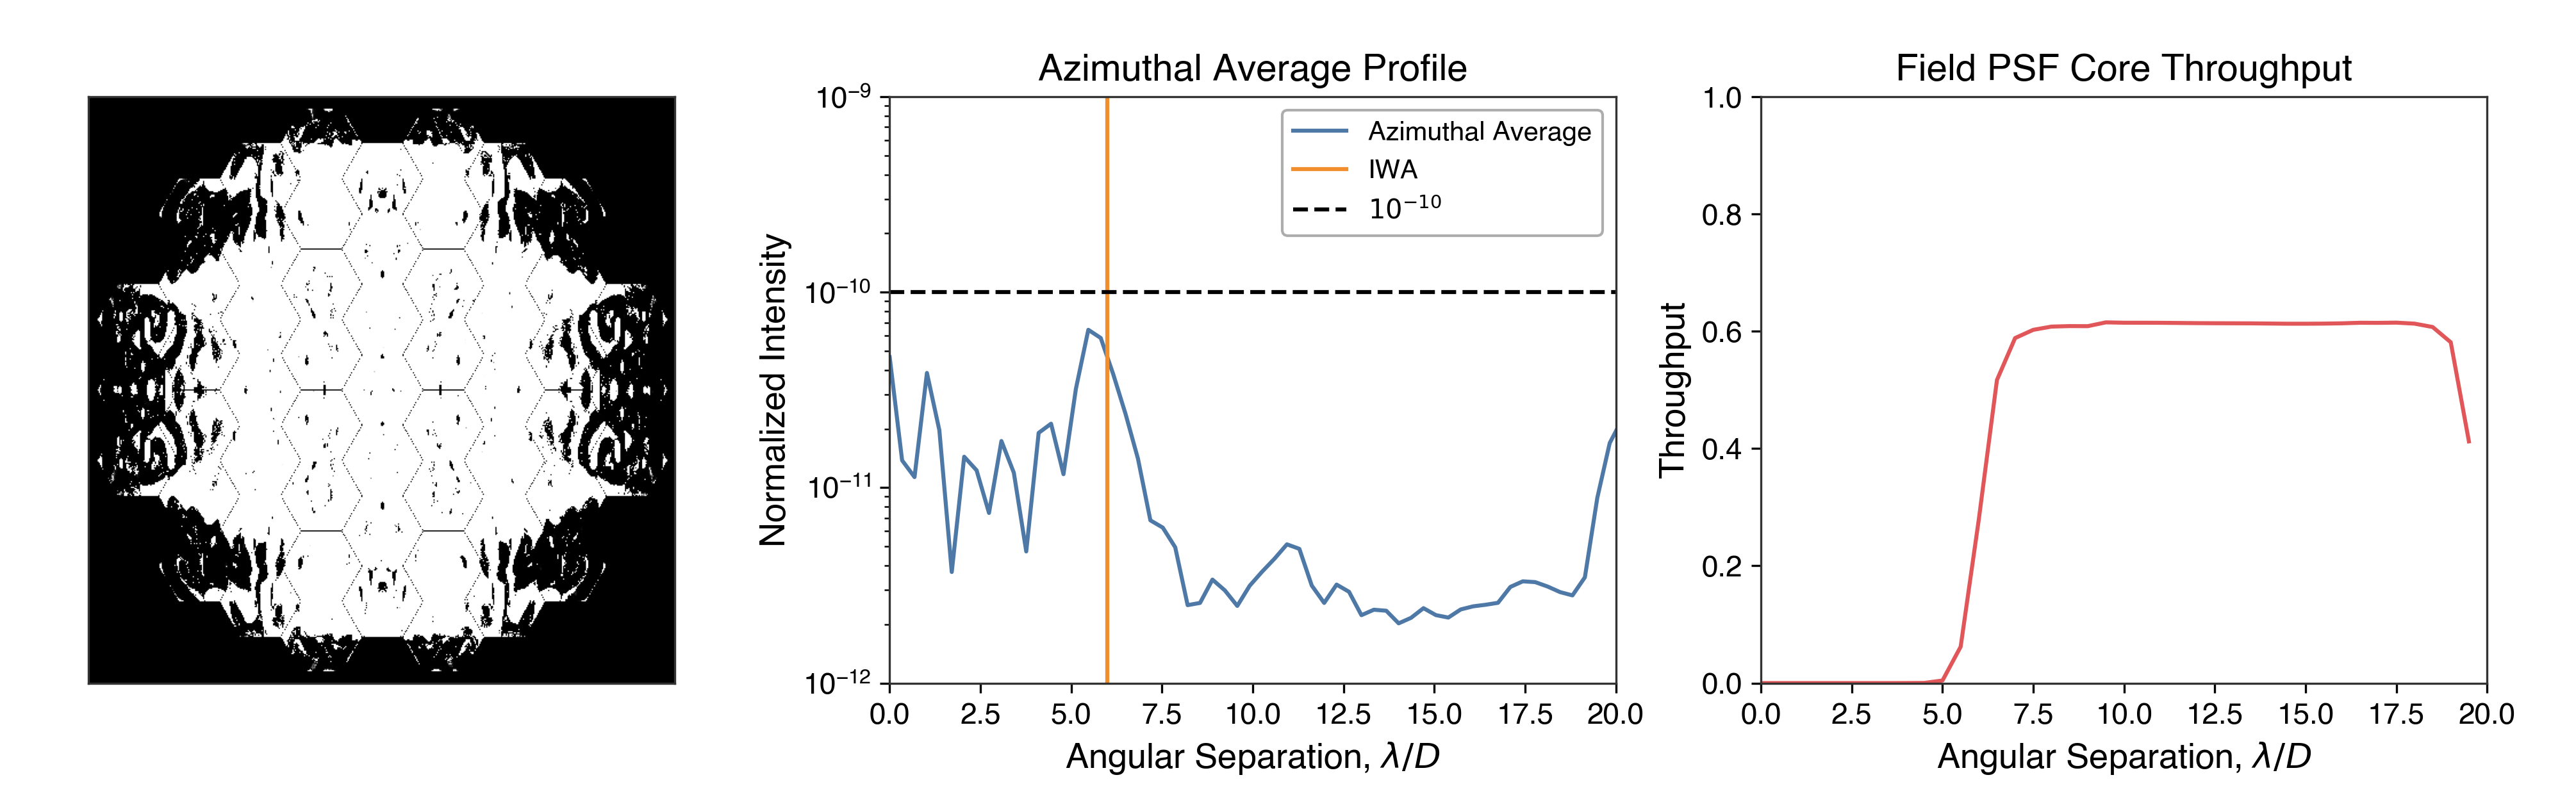
\includegraphics[width=\textwidth]{point_design.png}
    \caption{The starting point design that we use as a point of comparison for our excercises in throughput maximization. (Left) The APLC pupil apodizer result from our nonlinear optimization. (Middle) The azimuthally averaged radial profile in normalized intensity at the coronagraphic focal plane. (Right) The core throughput, a ratio of the encircled energies between the coronagraphic PSF and the non-coronagraphic PSF as a function of angular separation. We observe $60\%$ core throughput for a coronagraph that reaches $10^{-10}$ normalized intensity at the inner working angle. In comparison to Por's work on APLC design\cite{Por_2020} that achieve $10-15\%$ core throughput at half the IWA ($3\lambda/D$), the relaxed IWA accessible in the UV grants us 4-6$\times$ the throughput.}
    \label{fig:point_design}
\end{figure}

\section{Is there an optimal bandwidth for UV APLCs}
\label{sec:bandwidth_survey}
One avenue for maximizing the ``throughput" of UV APLCs is to increase the bandwidth of the coronagraph. While coronagraphs require modest bandwidths of $\approx 10-20\%$ because of chromatic wavefront error, in principle, a UV APLC could be optimized to support a larger bandwidth if the wavefront sensing and control can support it. We begin answering this question with another APLC design survey, where the core throughput is evaluated in $2\%$ increases of bandwidth beginning at $2\%$and ending at $50\%$. 

\begin{figure}
    \centering
    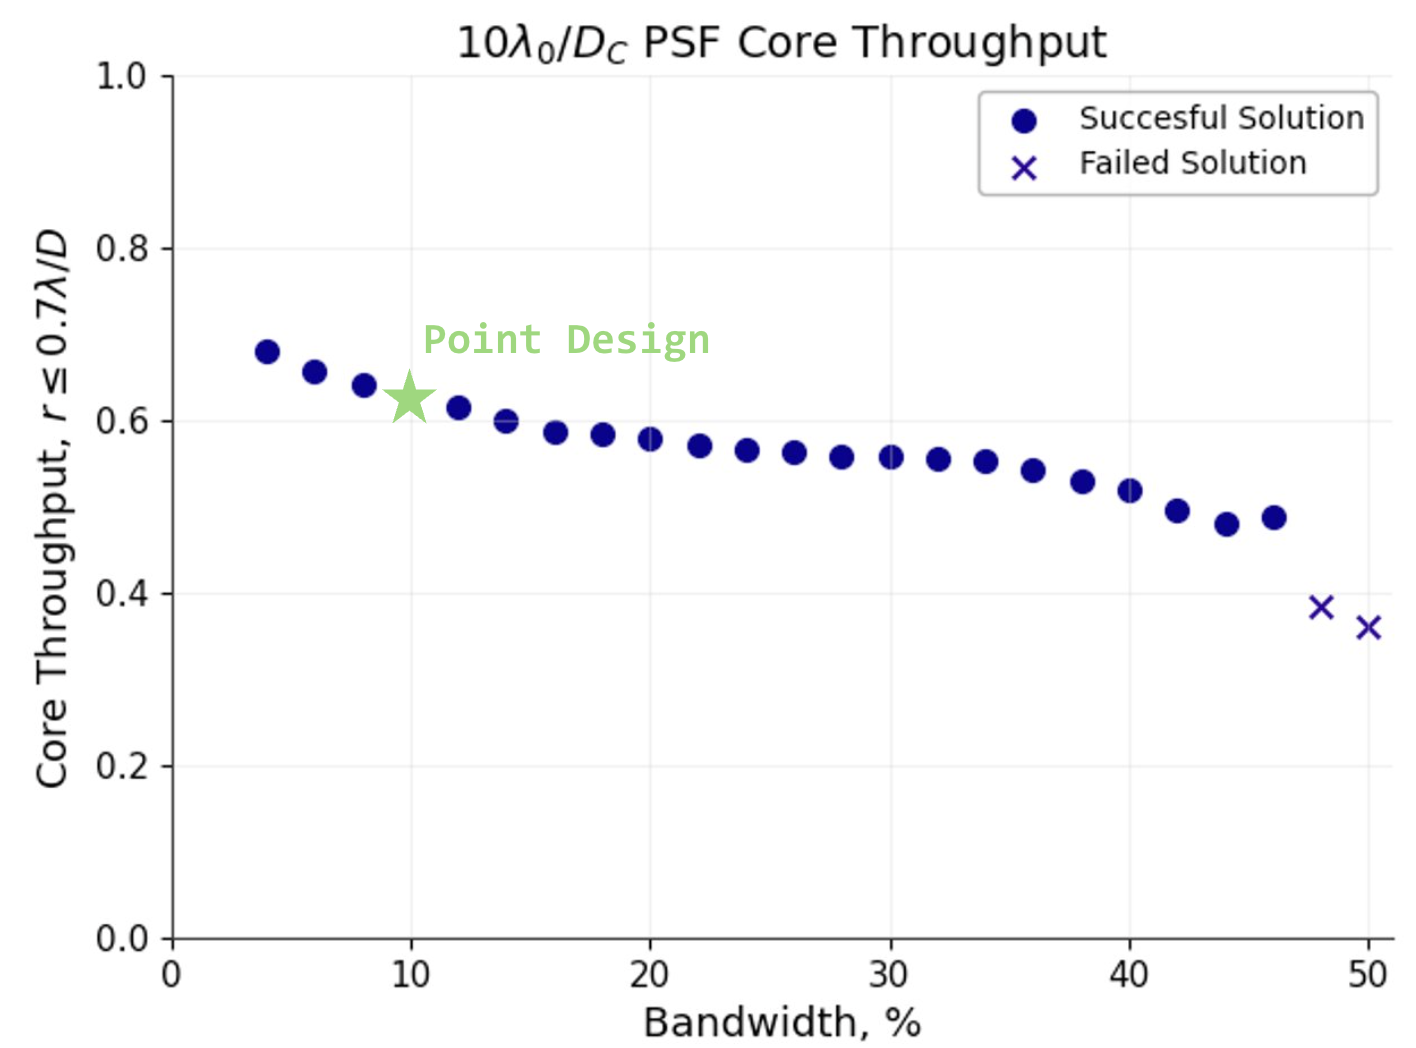
\includegraphics[width=0.5\textwidth]{bw_survey.png}
    \caption{Survey of the core throughput at $10 \lambda_C/D_C$ of APLCs at different bandwidths. Beginning at $2\%$ and ending at $50\%$, spaced in $2\%$ increments. We find that at an inner working angle of $6 \lambda/D$, the core throughput is not a strong function of the bandwidth. Only at the $48\%$ and $50\%$ solutions did the solver fail to find an acceptable solution. These solutions were grayscale, and had a percipitous drop in throughput. However, these data suggest that a $46\%$ bandwidth UV APLC will only suffer from a $\approx 5\%$ decrease in core throughput, and more than make up for this loss with $4.6\times$ more photons than the point design. This of course neglects the important problem of wavefront sensing and control in such a wide bandwidth, which was not considered for these calculations. We only suggest that the APLC design is not bandwidth-limited, and this can be a degree of freedom for future investigators to use to maximize throughput.}
    \label{fig:bw_survey}
\end{figure}

\subsection{How did the aberration sensitivities change?}
Important to consider when changing the APLC design is how the response to low-order aberrations changes. The increased IWA offers us.

\section{Do Hexagonal or Circular lyot stops yield higher throughput results?}
\label{sec:ls_survey}
\textcolor{red}{Open aperture, erode aperture edges}
Erode aperture edge until open area is the same! 

\subsection{Did aberration sensitivities change?}

\section{Conclusions}
\label{sec:conclusions}

\section{Appendix A: Gradient Backpropagation for the Augmented Lagrangian Method}
To democratize this analysis we carry out the algorithmic differentiation by hand and return the mathematical models to the reader to be implemented in the programming language of their choice. Por\cite{Por_2020} revolutionized coronagraph design by implementing the Augmented Lagrangian Method (ALM) for APLC and PAPLC optimization. Here we work out the reverse-mode algorithmic differentiation of the ALM so that it can be included in other optimization routines. This is the same RMAD algorithm we implement in \texttt{dygdug} as an option for coronagraph optimization.

The ALM expresses the loss function via a sum of the objective function $f$ with $i$ quadratic penalties $c_i$ imposed on the optimization, as shown in Equation \ref{eq:augmented_lagrangian},

\begin{equation}
    \mathcal{L}(x) = f(x) + \frac{1}{2}\sum_i^m \mathbf{\Phi}(c_i(x); \lambda_i, \rho_i),
    \label{eq:augmented_lagrangian}
\end{equation}

\begin{equation}
     \mathbf{\Phi}(c_i(x); \lambda_i, \rho_i) = 
        \begin{array}{l l}
             
     -\lambda_i \circ c_i(x) + \frac{1}{2}\rho_i c_i(x)^2 & \texttt{if}\phantom{o} c_i(x) \leq \lambda_i/\rho_i  \\
     -\lambda_i^2/2\rho_i & \texttt{if}\phantom{o} c_i(x) > \lambda_i/\rho_i
        \end{array}
\end{equation}

where $\lambda_i$ is the eponymous ``lagrange multiplier", $c_i(x)$ is the scalar constraint function, and $\rho_i$ is the penalty parameter. By observation, we know that the case where the constraint is satisfied $c_i > \lambda_i/\rho_i$, the constraint function is constant. Therefore, the gradient is zero-valued in this case and we only need to back-propagate the quadratic penalty function when the constraint is violated. We refer to the evaluated constraint function as $\mathcal{C}=c_i(x)$, and express the penalty function in Equation \ref{eq:penalty_function}

\begin{equation}
    \mathbf{\Phi} = \lambda_i \circ \mathcal{C} + \frac{\rho_i}{2} \mathcal{C}^2.
    \label{eq:penalty_function}
\end{equation}

The partial derivative of $\mathbf{\Phi}$ with respect to $\mathcal{C}$, $\overline{\mathcal{C}}$, is then given by Equation \ref{eq:penalty_gradient}. This quantity is multiplied by the partial derivative of 

\begin{equation}
    \overline{\mathcal{C}} = \rho_i \circ \mathcal{C} - \lambda_i
    \label{eq:penalty_gradient}
\end{equation}


\acknowledgments % equivalent to \section*{ACKNOWLEDGMENTS}       
 
J.N.A was supported by NASA through the NASA Hubble Fellowship grant \#HST-HF2-51547.001-A awarded by the Space Telescope Science Institute, which is operated by the Association of Universities for Research in Astronomy. Resources supporting this work were provided by the NASA High-End Computing (HEC) Program through the NASA Advanced Supercomputing (NAS) Division at Ames Research Center. Use was made of computational facilities purchased with funds from the National Science Foundation (CNS-1725797) and administered by the Center for Scientific Computing (CSC). The CSC is supported by the California NanoSystems Institute and the Materials Research Science and Engineering Center (MRSEC; NSF DMR 2308708) at UC Santa Barbara.

% References
\bibliography{report} % bibliography data in report.bib
\bibliographystyle{spiebib} % makes bibtex use spiebib.bst

\end{document} 
